\documentclass[12pt]{article}
\usepackage{cite}
\usepackage{graphicx}
\usepackage{setspace}
\usepackage{indentfirst}
\usepackage{listings}
\usepackage{mathpazo}

\begin{document}

%Title page

\begin{titlepage}
    \begin{center}
        \vspace*{0.5cm}
        
        \begin{doublespace}        
        \textbf{\Large Navigating Articles of News Websites Using a Near Real-Time Web Metrics Visualization}
        \vfill


        A Thesis in the Field of Information Technology \\
        In Partial Fulfillment of the Requirements \\
        For a Master of Liberal Arts Degree
        
        \vspace{0.8cm}
        
        Harvard University \\
        Extension School \\
        May 28, 2014        
        
        \vspace{1.5cm}
        
        \textbf{Alain Ibrahim} \\
        4551 Interlachen Ct. Unit I \\
        Alexandria, VA 22312 \\
        Cell: (703)932-9397 \\
		alain\_ibrahim@hotmail.com \\   
        Proposed Start Date: May 2014 \\
        Anticipated Date of Graduation: May 2015 \\
        Thesis Director: Alexander Lex \\
		\end{doublespace}        
        
        \vfill
         
    \end{center}
\end{titlepage}

\tableofcontents

\vfill

%Abstract

\section{Abstract}

Current prominent web traffic analytics systems such as Google Analytics convey traffic per website, given certain filtering criteria. Though, such systems are typically geared to system administrators who use the data to identify patterns and possibly assist management in strategy making. For news sites, this may mean analyzing the traffic on a news article, where most of the readers came from, etc. The end users, however, will at best see metrics such as social likes and shares. But, what if we could provide the end users a near real-time metrics map of the entire news site they are visiting? What if they could navigate more efficiently, as opposed to having to follow the common front page layout dictated by the news editors? This system is what I plan to build – a web-based, interactive visualization that conveys the near real-time metrics of a select news site.
First off, I plan to build a server-side library that can be included into any website or web application. This library would hook into a relational database and would efficiently capture the hits (possibly inclusive of IP addresses, geo locations, etc.) against the given news site.
My second step involves building the "business logic" of the data and information that I want to capture. This includes algorithms that produce the refined data and metrics to be ultimately communicated to the end user.
My final step is to build a central interactive visualization that shows near real-time user web traffic in each of the registered articles of the given news site. In the proposed scenario, the user will:
\begin{itemize}
\item See an overview map of the news site’s articles.
\item Filter traffic based on available data, such as the user’s geographic location.
\item Possibly see the average read time of a select article. The overall goal is to have a more personal browsing experience in the midst of all the "guided" text and hyperlinks.
\item Navigate to the article of interest by clicking on its visual representation.
\item Obtain details on demand for a given news article by hovering over its visual representation.
\end{itemize}

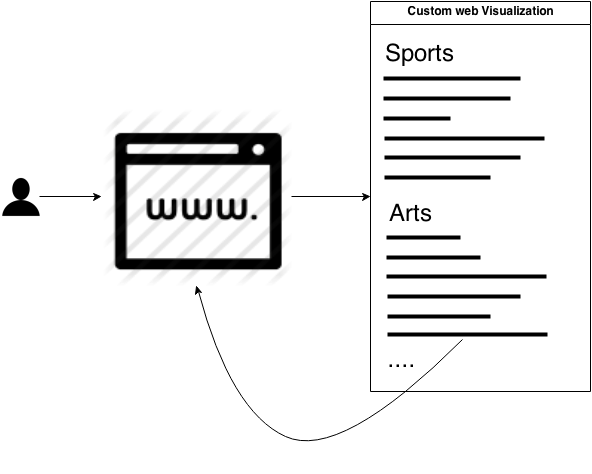
\includegraphics[scale=0.6]{img/overall_chart}

\noindent\textbf{Diagram 1 -- A general overview of the proposed system. In this diagram, the user visits a news site; from within, the user loads an interactive and navigable web visualization (the above is an impression). The visualization conveys visual encodings of the articles, which link back to the articles themselves.}

\vfill

\section{Thesis Project Description}
On the server side scripting end, I will build php classes that will be included in the top of the news site's file(s). The code will register every visiting IP address. A hit/visit can be potentially defined as a unique IP address hitting the news site near real-time, thereby countering against bots and maximizing the accuracy of the readings. Another way of defining a hit would be to utilize HTML5’s LocalStorage. In this scenario, the server-side PHP script would issue a unique token per client browser. The active tokens would then be managed in a database to keep track of connecting clients. An alternative method to register hits is to utilize HTML5’s WebSocket on the client side, matched with a socket server on the server side.

I will build the relational database using normalization techniques and principles. I plan to also apply indexes where applicable.

\noindent{Here are the technologies that I plan to use:}
\begin{itemize}
\item MySQL relational database
\item PHP for server-side scripting
\item HTML 5, CSS3, and JavaScript for client-side design and implementation
\item Third party client-side libraries to ameliorate the final design and to facilitate the visual implementation. I am specifically considering D3.js
\end{itemize}

I plan to capture near real-time web traffic – for this project, this means the last 12 hours of user activity. To facilitate the visualization creation process, I plan to use the D3.js (Data-Driven Documents) Javascript library. On the markup and structural side, I may use <canvas>, <svg>, or just plain HTML. The domain at hand will be that of \textbf{news media online}. As for the resultant visualization, the design will be tailored to enable one primary and one secondary task:
\begin{itemize}
\item Primary task - To Navigate a news website based on its traffic metrics
\item Secondary task - To analyze web traffic metrics in near real-time
\end{itemize}

The resulting visualization will be a separate html page that is invoked through the website through a clickable button. This page will span across the width and height of the browser.

\noindent{In terms of interactivity, the said visualization should include the following:}
\begin{itemize}
\item Hovering over article elements in order to see previews of the articles (main image, text description, and some of the body’s text)
\item Clicking on an article’s visual encoding should direct the user to the actual article page, in a separate browser tab
\item A pane that enables the user to filter the data, and zoom (if needed)
\end{itemize}

\noindent{As for web traffic data being captured, here is a list of what I plan to attain, in order ascending difficulty:}
\begin{itemize}
\item Visitor hits to a given article
\item Geographical origin of the visitors to a given article
\item Average read time of a given article.
\end{itemize}

The final product will be geared towards the conventional news site structure, where categories are enumerated (e.g. sports, health, science, politics, etc.), and where articles are listed under their pertinent categories. The below sketches illustrate part of the user experience of the final visualization.\\

\noindent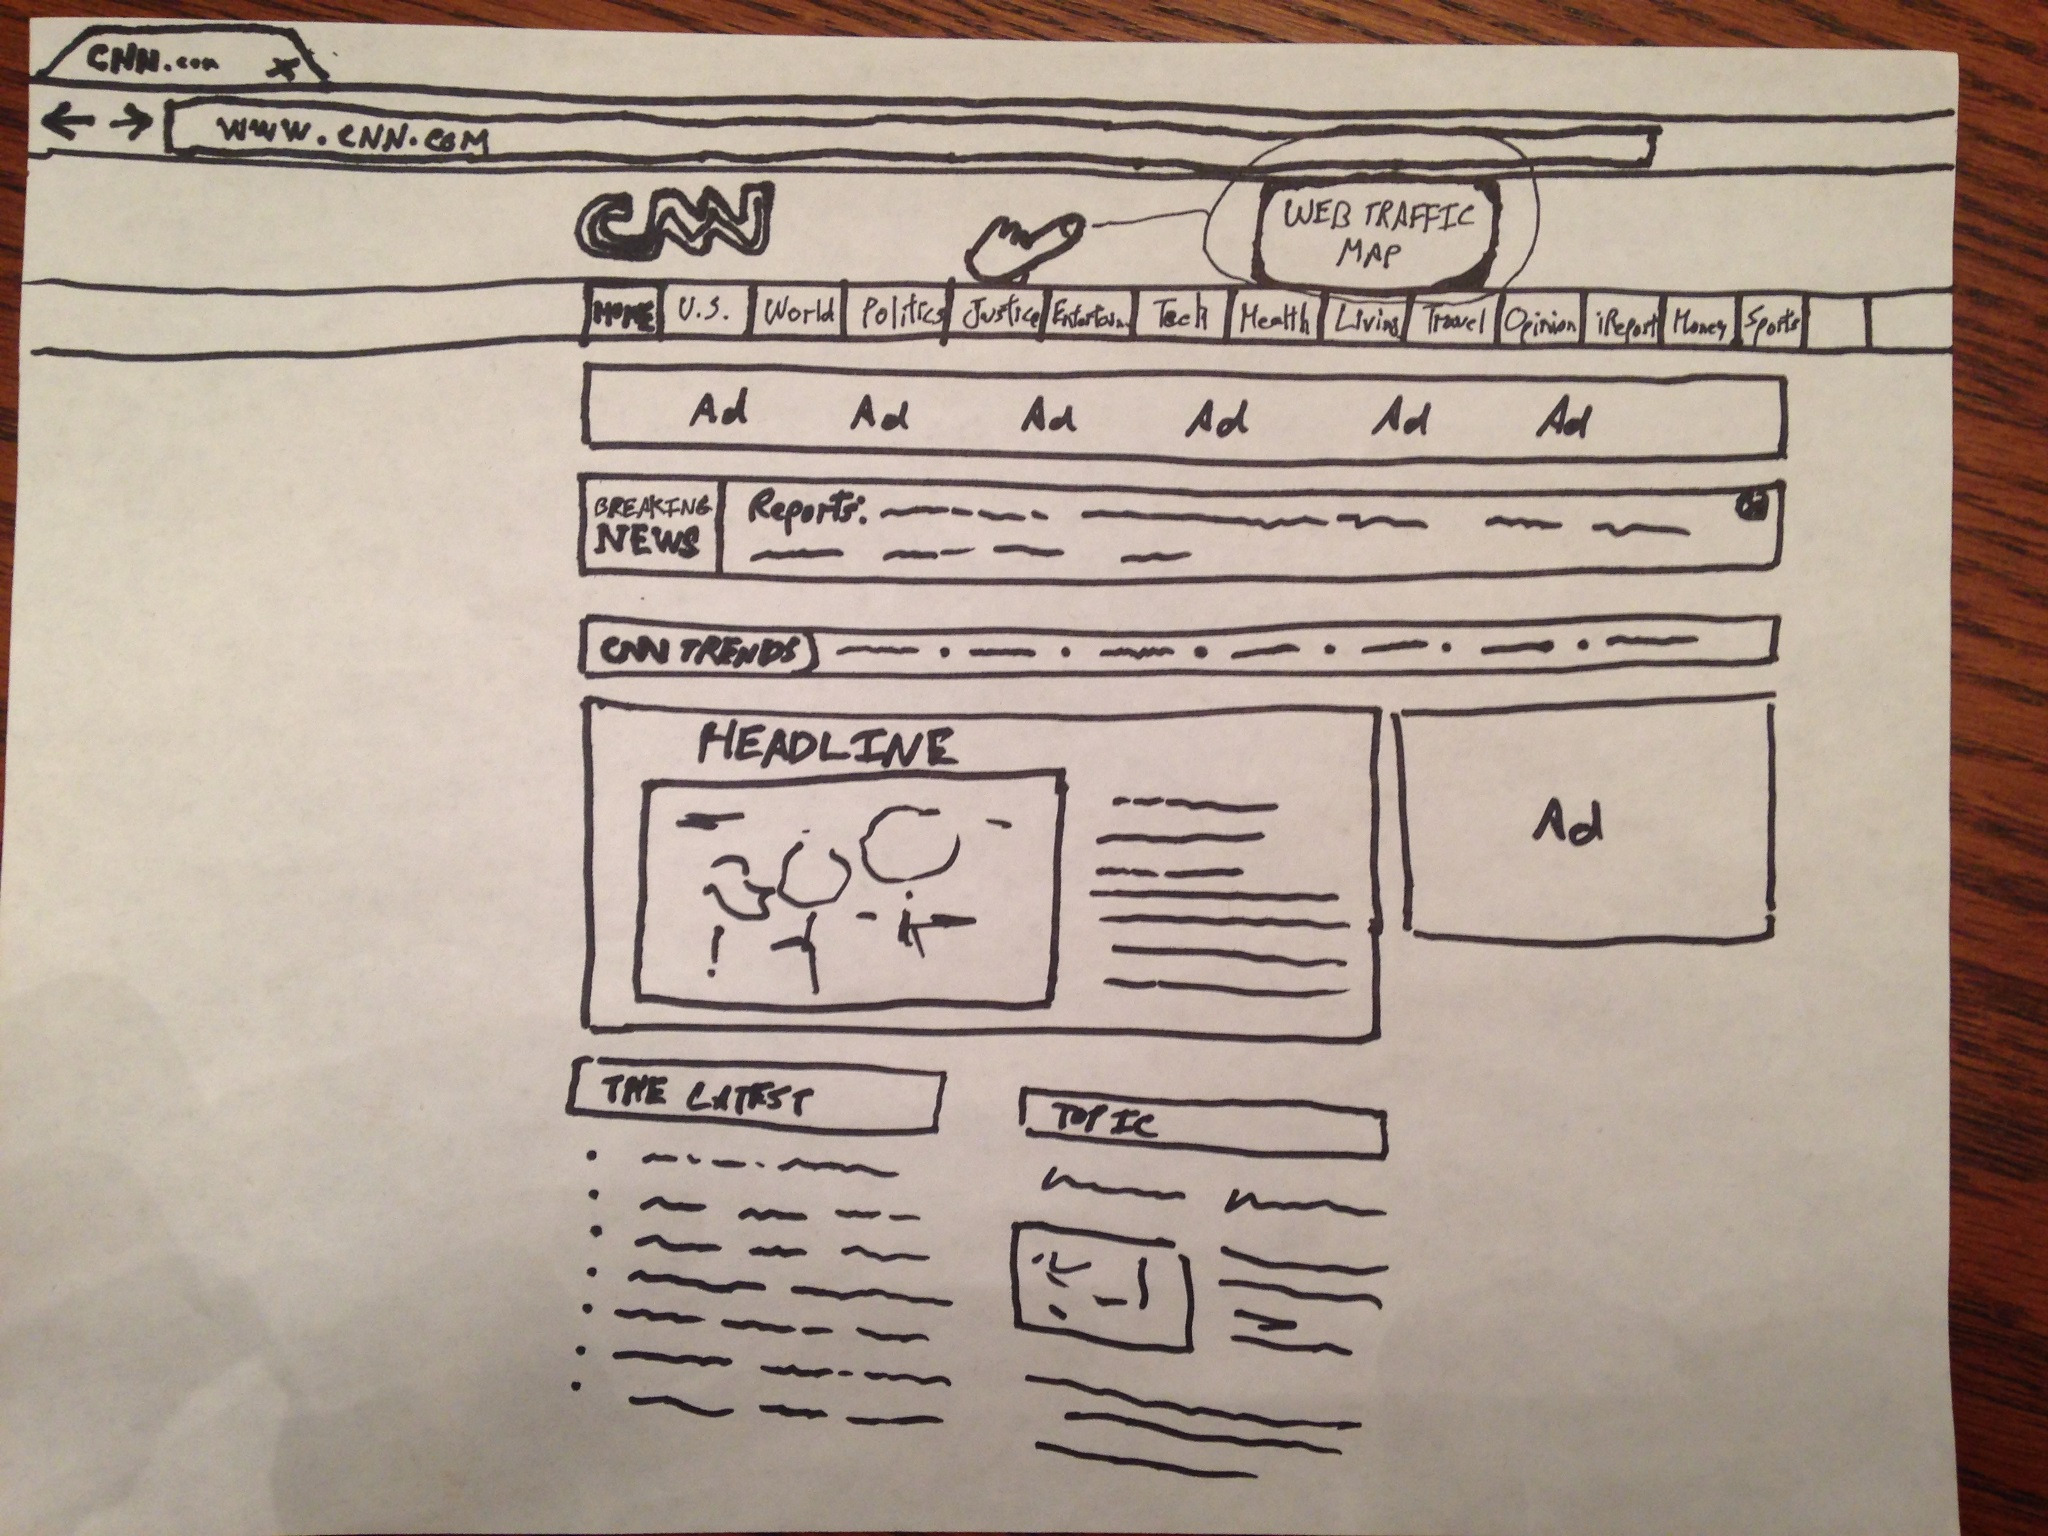
\includegraphics[scale=0.2]{img/cnn_example}
\noindent\textbf{Diagram 2 –- On a news site like CNN, for example, there would reside a link to the near real-time visualization.}

\noindent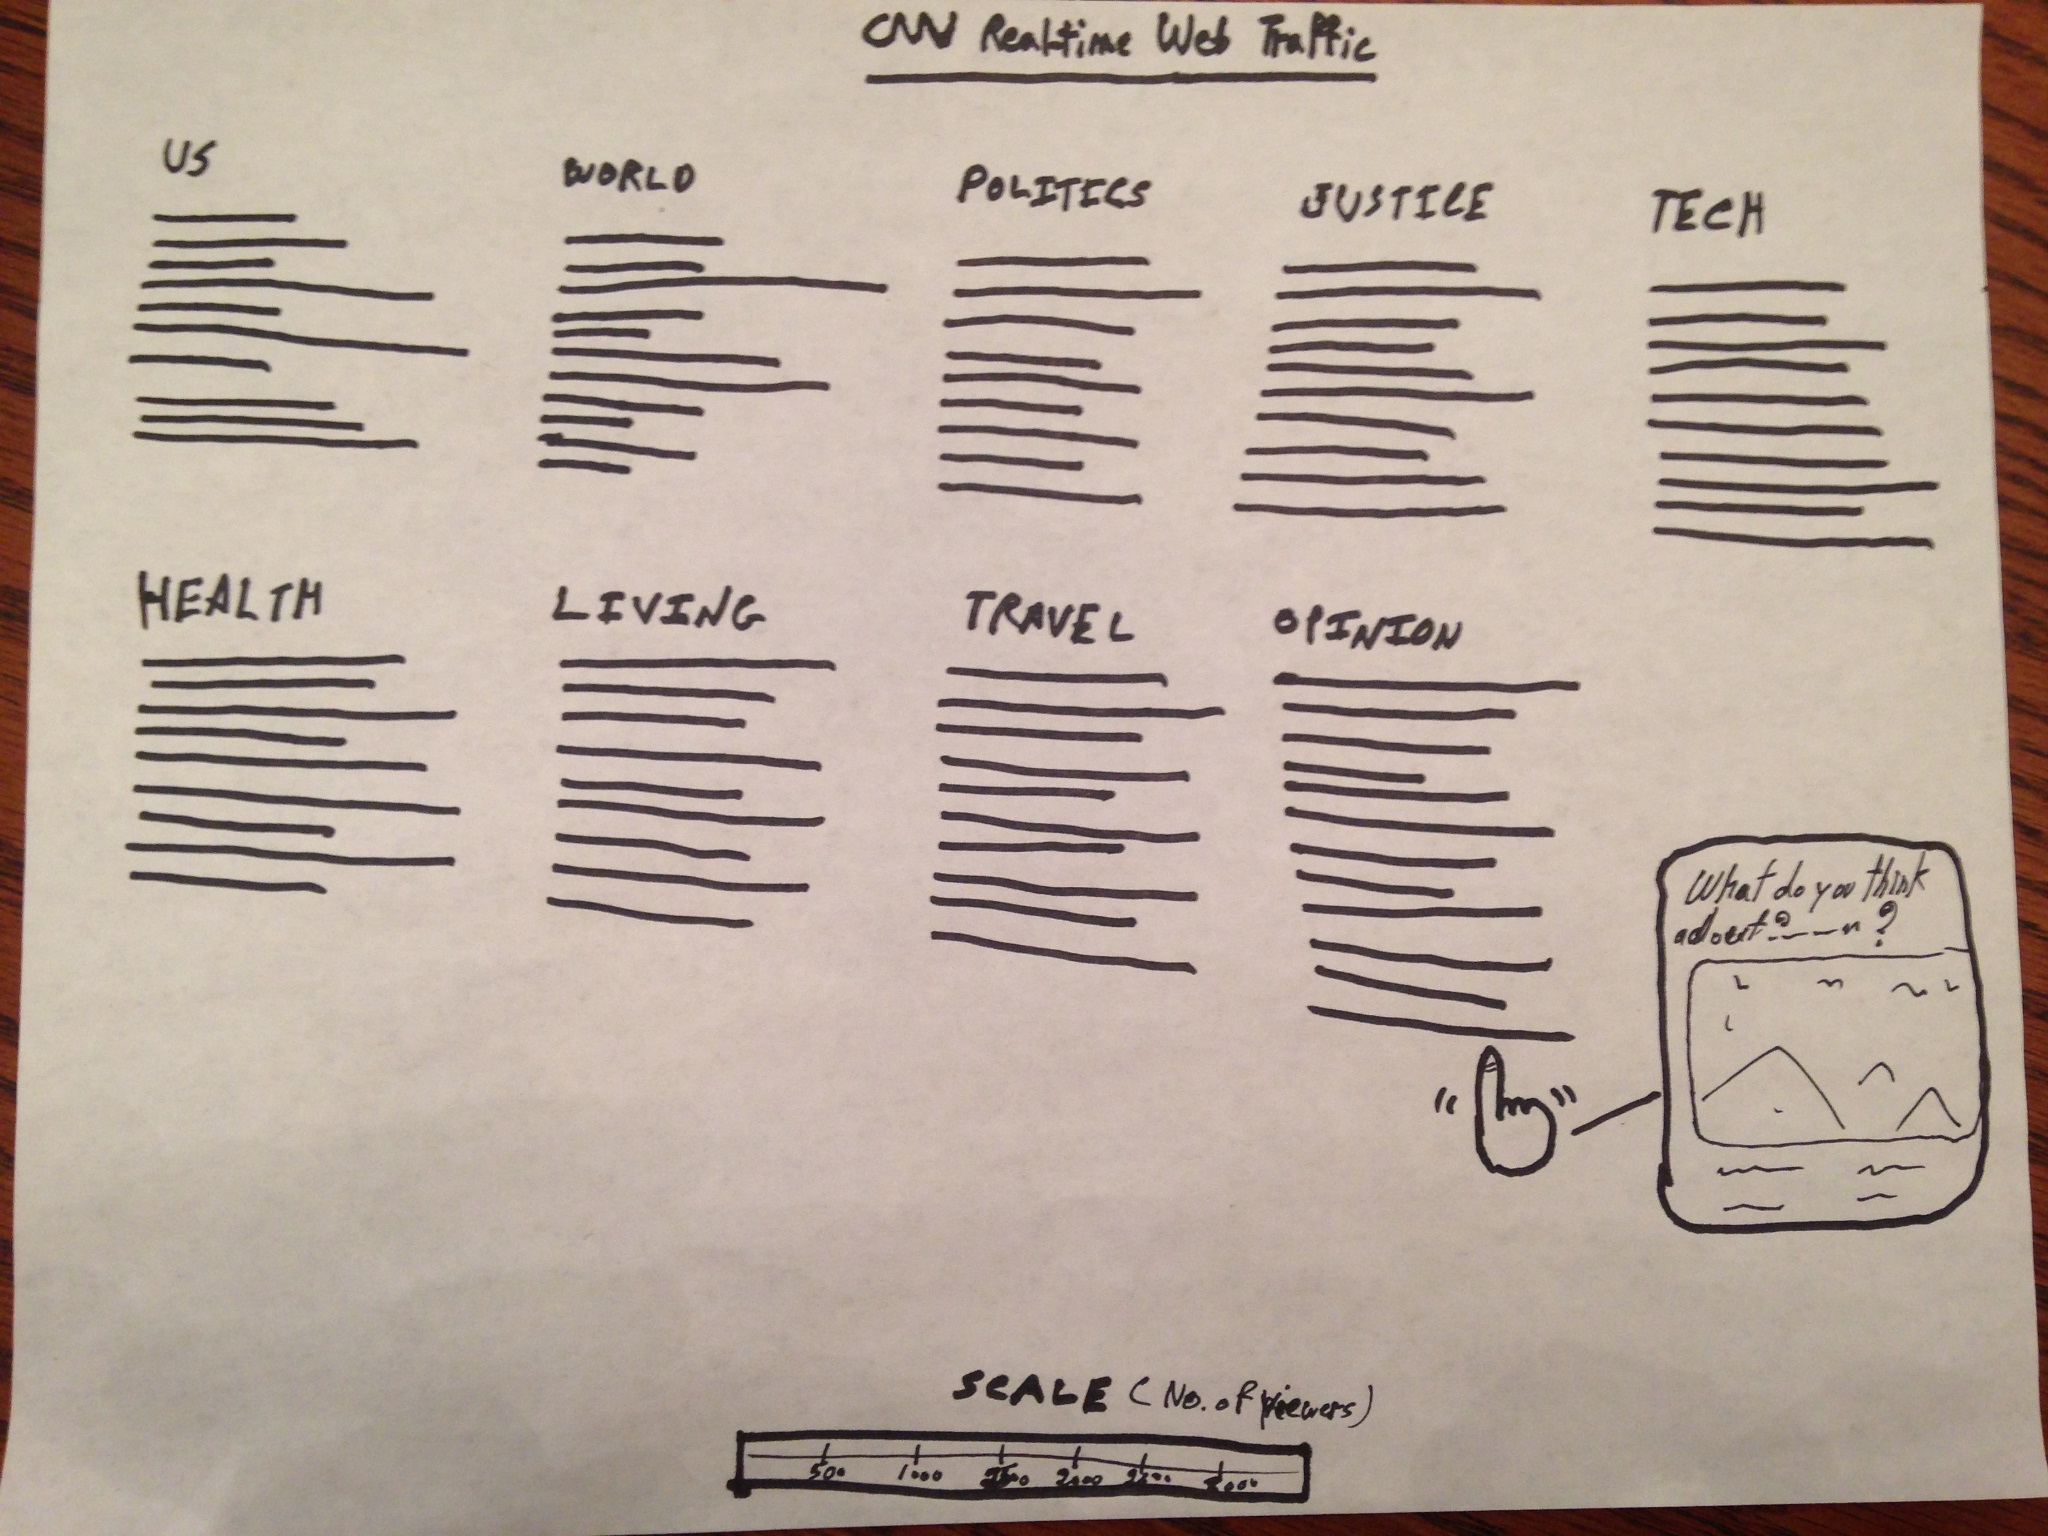
\includegraphics[scale=0.2]{img/cnn_categories}
\noindent\textbf{Diagram 3 –- A potential way of visualizing the near real-time traffic. Here, the articles are encoded by lines. Each line’s length signifies how much traffic a select article has. Hovering over said line/article invokes a details-on-demand window - showing the title, a picture snapshot, and perhaps some content from the article’s body.}

\noindent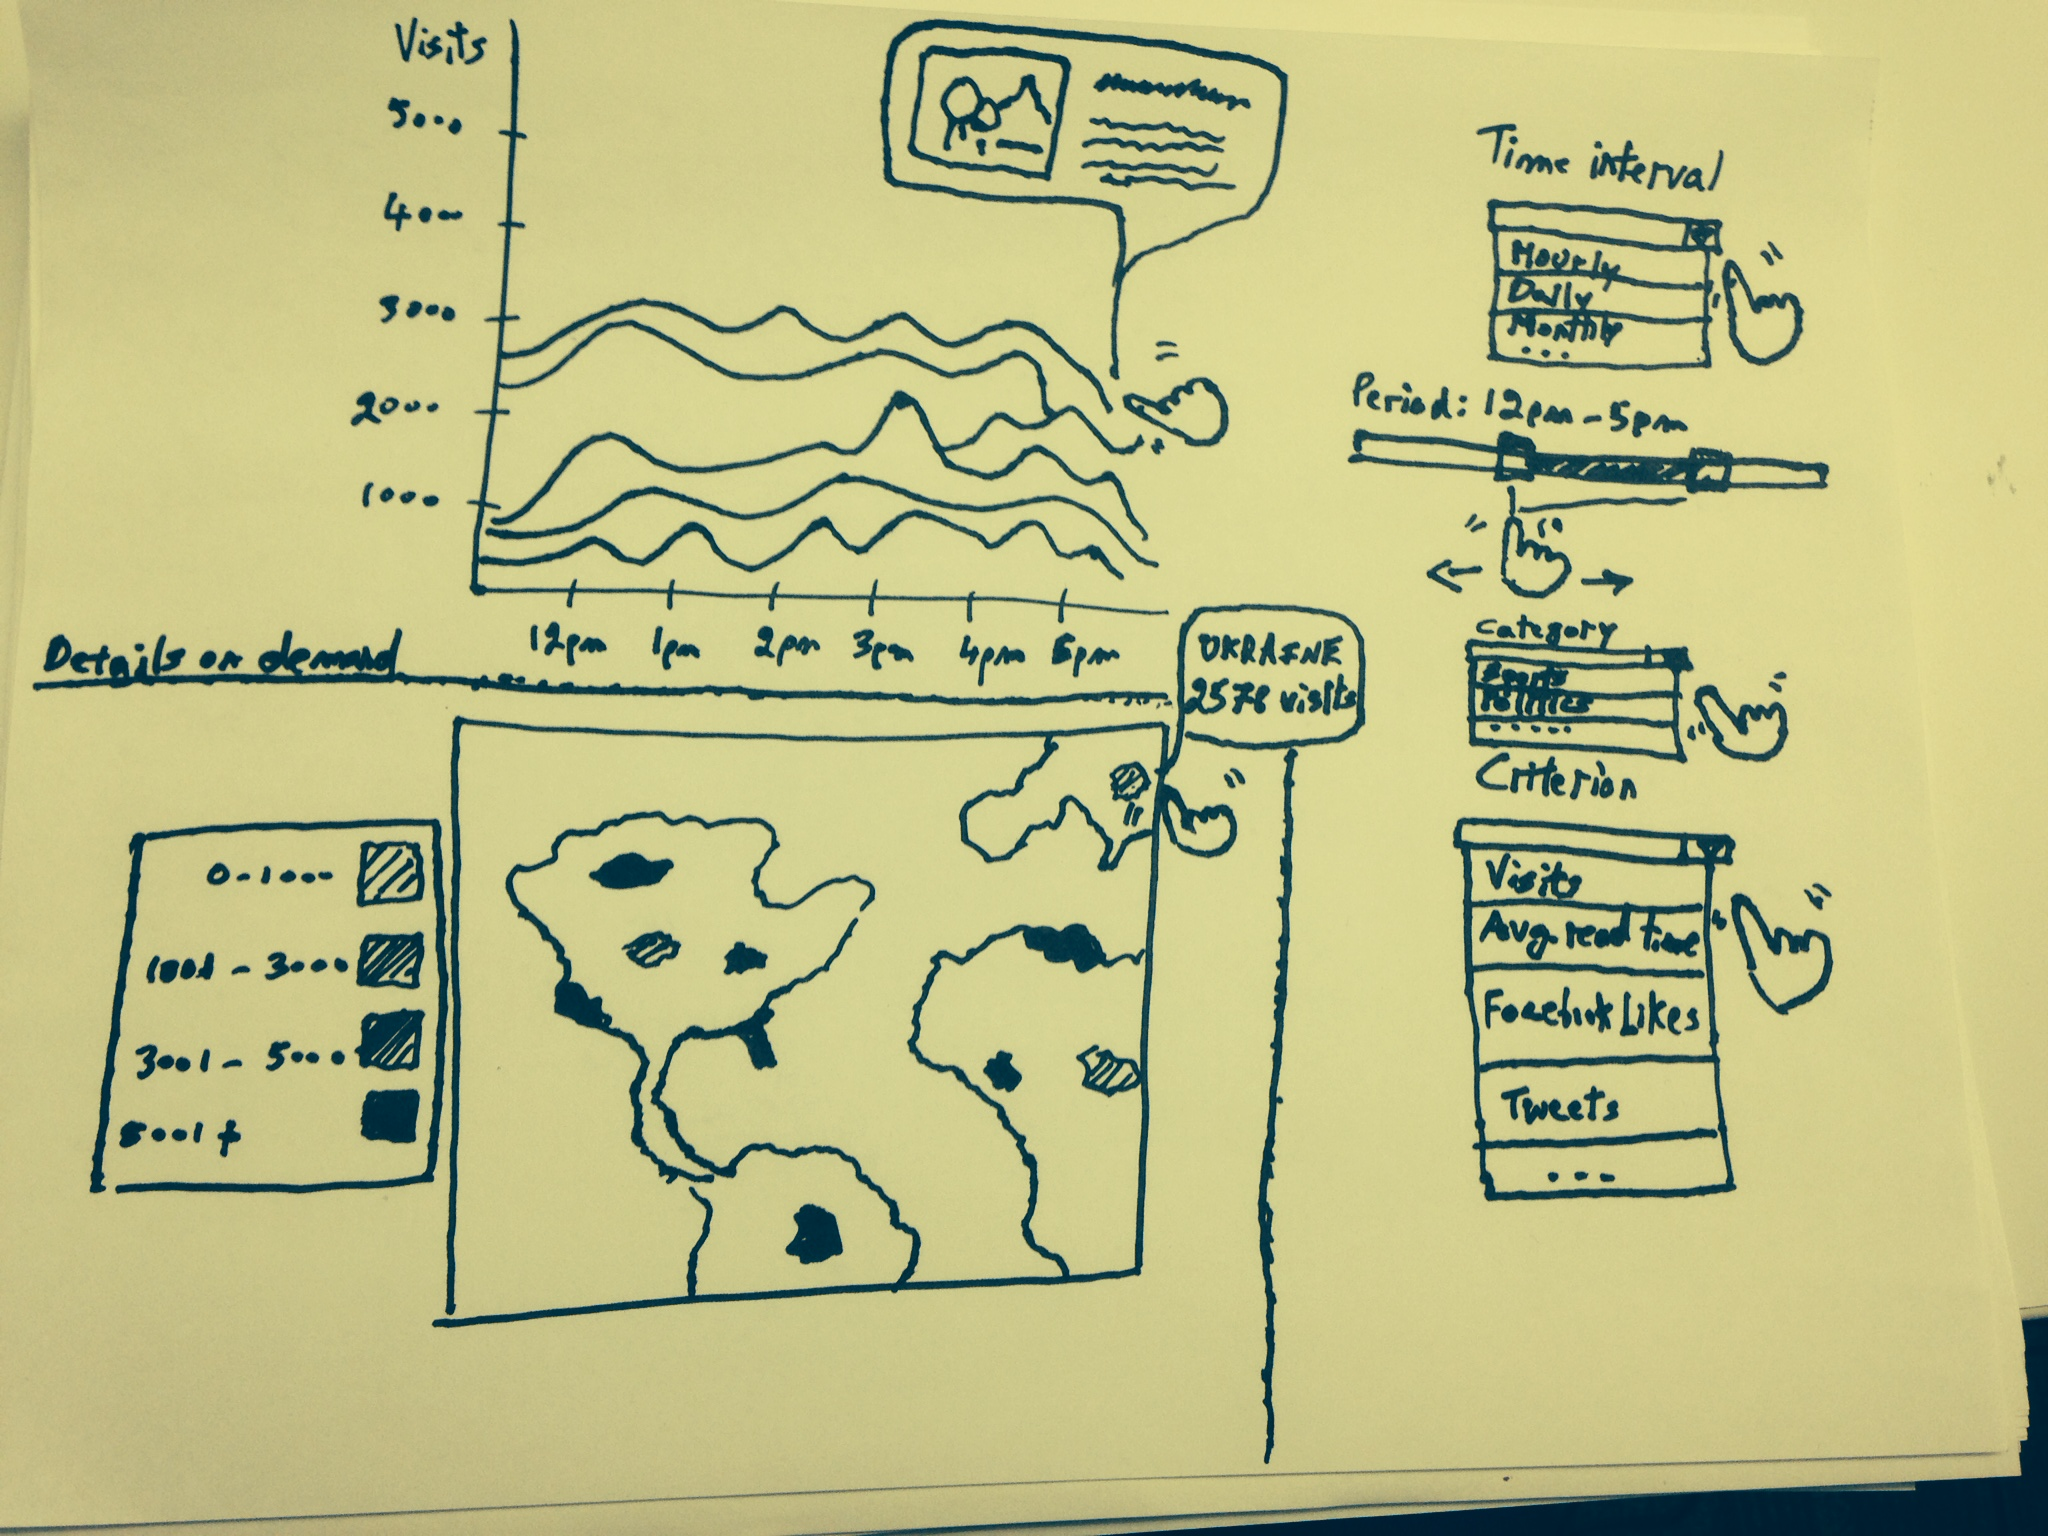
\includegraphics[scale=0.2]{img/overall_viz}
\noindent\textbf{Diagram 4 –- A conception of what the final artifact will look like. On the right resides the controls that allow the user to filter by time interval (daily, monthly, etc.), category (sports, business, politics, etc.), and the output criterion to measure (number of visits, average read time per article, facebook likes, etc.). The stream graph supports hover (details on demand) and click (to navigate to select article). Upon hovering over said article, the map should highlight the geographic origins of the visitors.}

\noindent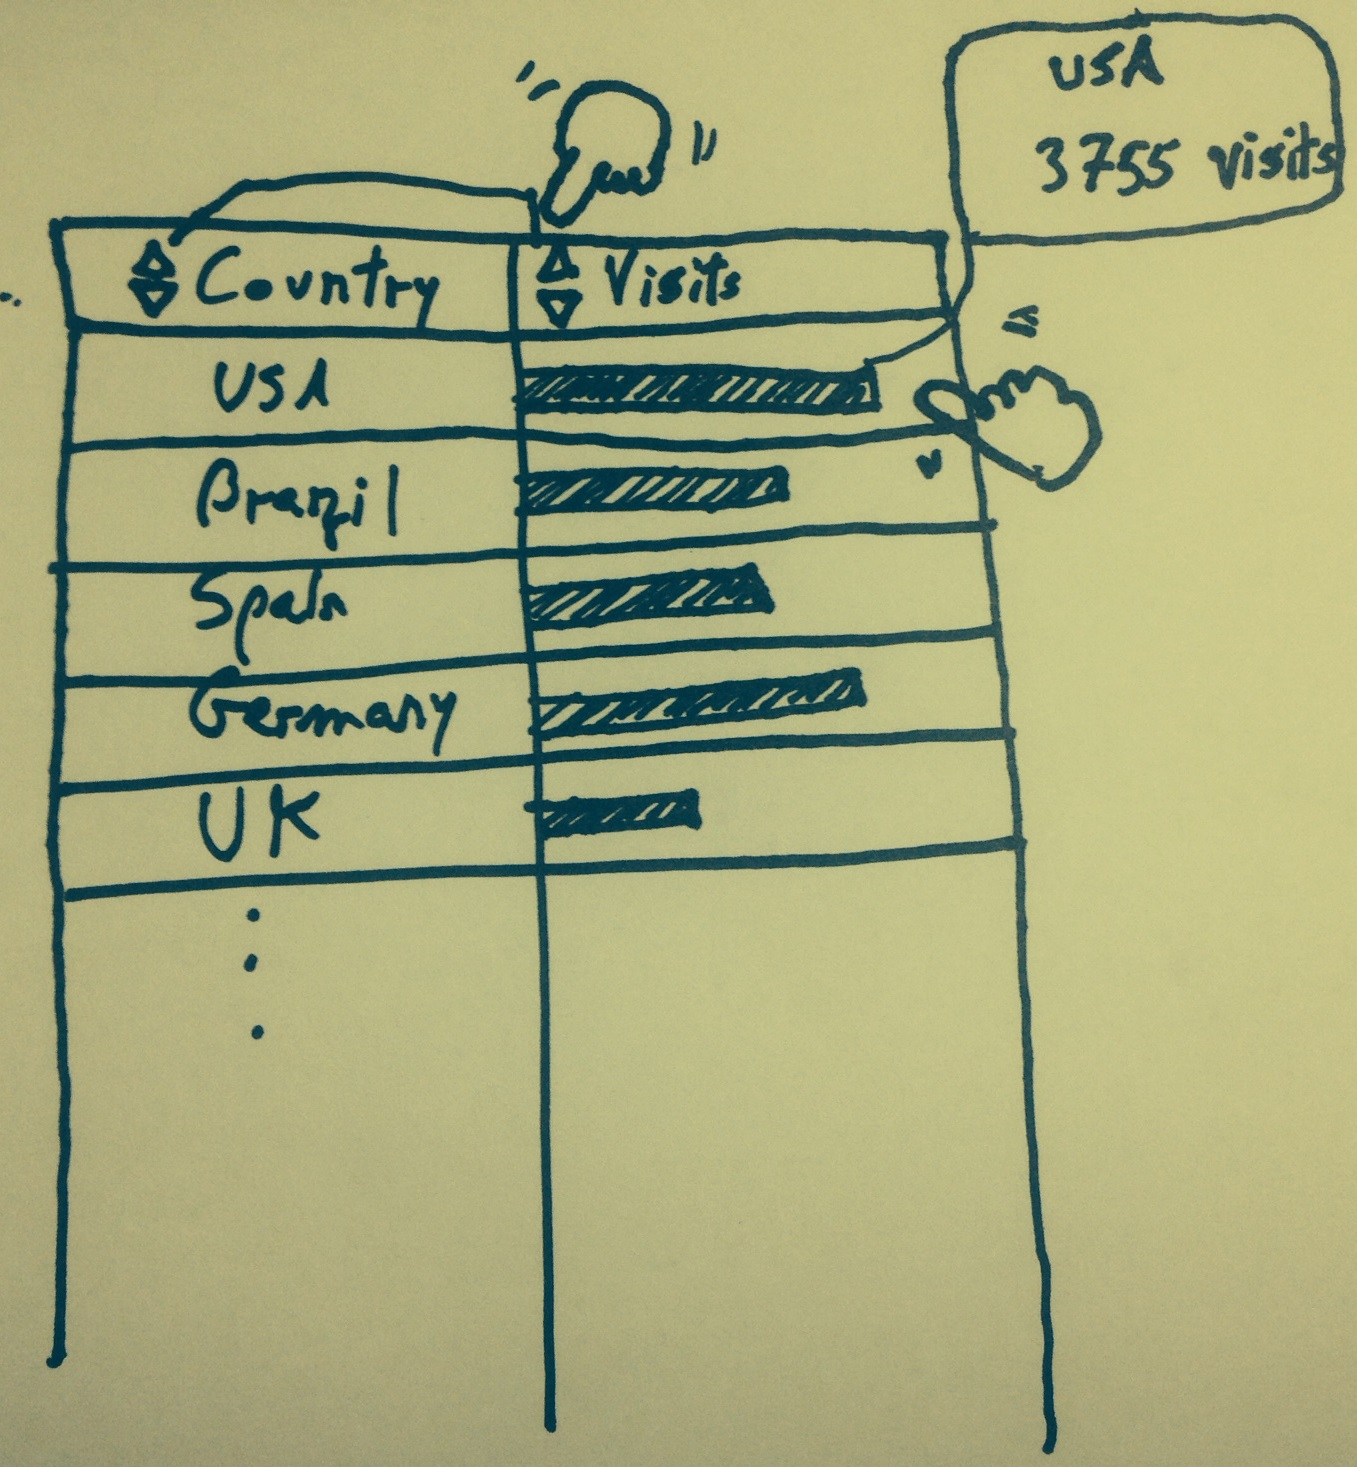
\includegraphics[scale=0.3]{img/table}
\noindent\textbf{Diagram 5 –- An alternative to the choropleth map in Diagram 4.} \\

My approach towards building the final product will entail the following, in chronological order:
\begin{enumerate}
\item Abstract the web traffic data that needs to be captured and develop the business model. In other words, I will have to define what data will be useful and how to algorithmically capture it
\item Build a relational database in MySQL around the results from 1)
\item Develop a server-side framework with PHP that would capture and retrieve the collected data
\item Research and experiment with different potential visualizations that could best fit 2)
\item Develop and implement the client-side visualization using D3. I anticipate capturing the data from the server side in JSON format
\end{enumerate}

\vfill

\section{Prior Work}
\subsection{Visualization}
Prominent researchers in the field of visualization have concocted logical constructs and approaches to designing and implementing visualizations. From a presentation standpoint, there is much emphasis on presenting the end user just enough visual data for the user to achieve the intended task of the visualization. Notions such as expressiveness \cite{schumann}, and increasing the data-to-ink ratio \cite{tufte} allude to the goal of building visualizations that can be efficiently processed by the human brain. Another criterion that is opted for is effectiveness. Enter the concepts of a domain and task \cite{munzner}. In the design phase, the builder needs to identify the domain that he/she is working with. A domain is a world of ideas and concepts that are abstracted under one umbrella. For example, human anatomy, software engineering, car racing, and pretty much any category one can think of is a domain. A domain gives rise to concepts, definitions, and a prebuilt library of shapes and colors by the convention of collective knowledge. For example, red in biology will signify blood whereas in the world of novels it may allude to romance. Knowing the domain aids the designer in introducing artifacts effectively and efficiently. On the other hand, the task refers to the “what” of the visualization. What is/are the goal(s) of the visualization? Is it to explore, analyze, extrapolate, etc.? Clearly identifying the task(s) of the visualization at hand solidifies the direction in which the designer encodes the visual variables (Bertin). Encoding refers to the idea of representing a quantitative or qualitative concept visually. The visual variables include position, size, shape, value, color, orientation, grain, and texture. At this point of the design process, most of the roadmap has been laid out for one to develop design sketches. Perhaps in the pre-Internet days, the implementation would have started here. Though, with the advent of mass computerization and global connectivity, a new ability has been introduced – that of interactivity. Interactivity has been broken down into the following \cite{cockburn}: Overview+Detail, Zooming, Focus+Context, details-on-demand, and cue-based systems.

Time is an essential component to web analytics, as it gives context to what is being measured. Although graphing change over time was attempted in the early A.D.s, the first known contemporary time series graph was published by William Playfair \cite{playfair}. Playfair was the father of the line graph and bar graph; it is important to note that these visual constructs were introduced in a time when they were not commonplace. Given this, a likely inclination towards visualizing temporal data would be to plot time against a Cartesian coordinates system. However, there is not a single model that accommodates all domains and tasks \cite{frank}. Thus, for the proposed visualization, time must be dealt with in the context of information systems in the news domain. As an employee of a news organization, I would like to take this opportunity to highlight the significant time units pertinent to news. Based on my observations of our news website and other similar entities’ websites, “news” refers to a recent occurrence, notably something that happened today. “Breaking News” typically refers to an event that happened within the current day and whose story under development. “Recent News” pertains to stories created within the last 1-3 days. As time approaches the coming year, decade, century, and millennium, news are then compiled and shown in representations such as “year/decade/century/millennium in review”. However, in order to achieve a meaningful representation in our visualization I must turn attention to the average lifetime of an article on a news website. Surely, a news article is only news when it is recent. Later references could be made to the said article when it is its “archives” period, but this would be only a temporal slice that would not be sufficient or useful when the task at hand is to have the user navigate based on article popularity. Thus, the time units (aka time granularities) that will support the task of the proposed visualization should be minutes and hours (for breaking news), and hours and days (for recent news) \cite{bettini}. Since I have interest in the general range of these units (e.g. 20 users looked at our article in the last minute/hour/etc.), I will need to use a discrete time scale \cite{goralwalla}. The output variables connected to time will mainly be number of hits, and may include figures such as the number of Facebook likes, number of Twitter tweets, and the average read time of an article.

\subsection{Existing web metrics systems}
What I plan to build is novel in that there is no current navigable tool that visualizes near real-time traffic on news sites. It should not only convey near real-time web traffic, but should also allow one to view metadata upon hovering over the selected article's representation, and should allow the user to directly navigate to it by clicking.\\
Here are a few systems that I found which deal with visualizing web metrics: \\

\noindent\textbf{Flow (http://www.webresourcesdepot.com/beautiful-free-website-traffic-visualization-application-flow/)} \\
\noindent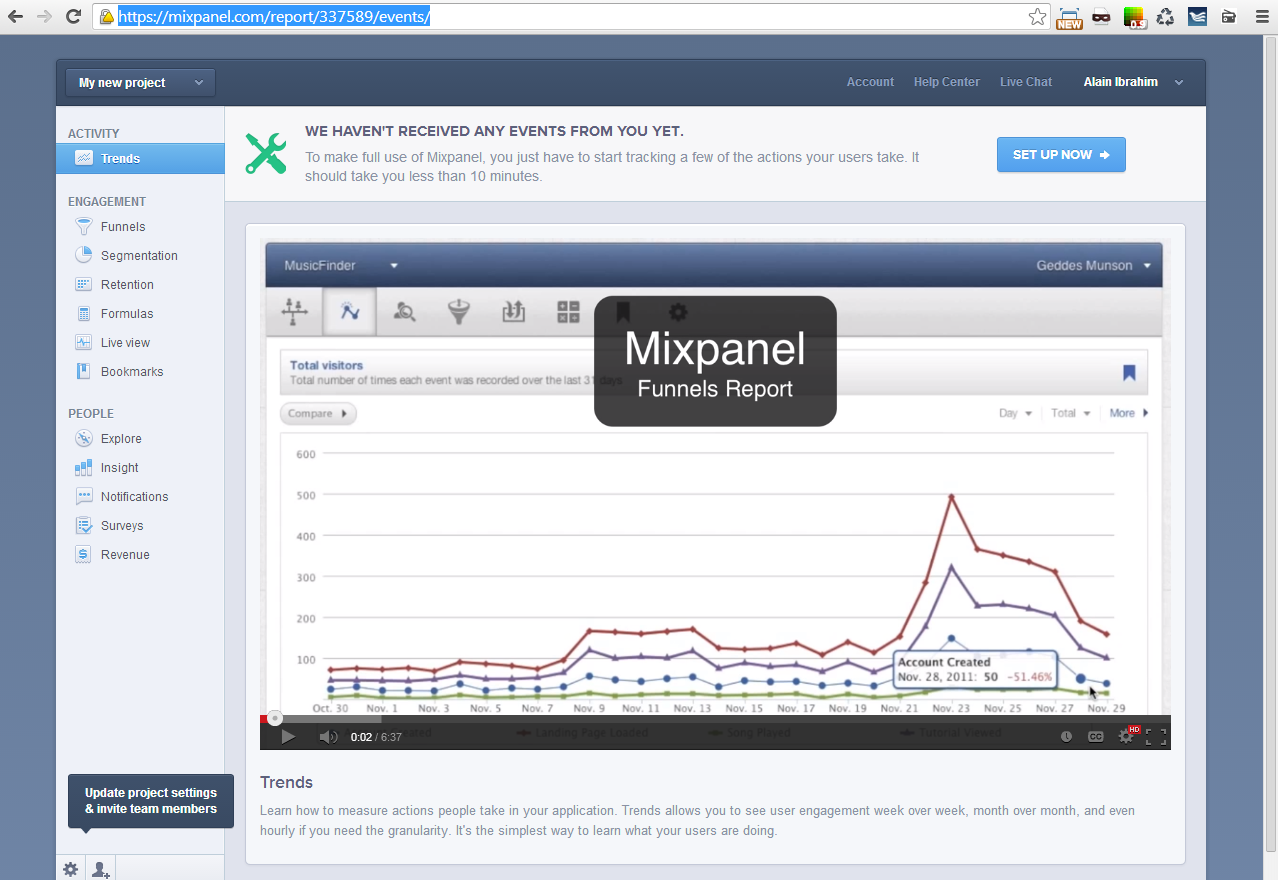
\includegraphics[scale=0.45]{img/flow}
\noindent\textbf{Diagram 6 –- Shows a line graph that measures the number of hits on the y axis, and date on the x axis for select categories on a given website.} \\

While this can be useful in providing some feedback to the news site’s administrators, it does not provide detailed insight to the articles in a given news site. The below screenshot demonstrates another visualization part of Flow. \\
\noindent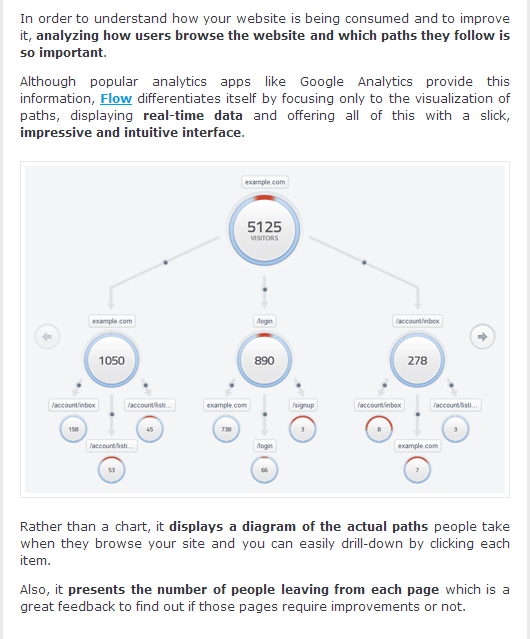
\includegraphics[scale=1]{img/flow1}
\noindent\textbf{Diagram 7 –- A visualization showing near real-time hits in sections of a given website.} \\

\noindent\textbf{Google Analytics} \\
\noindent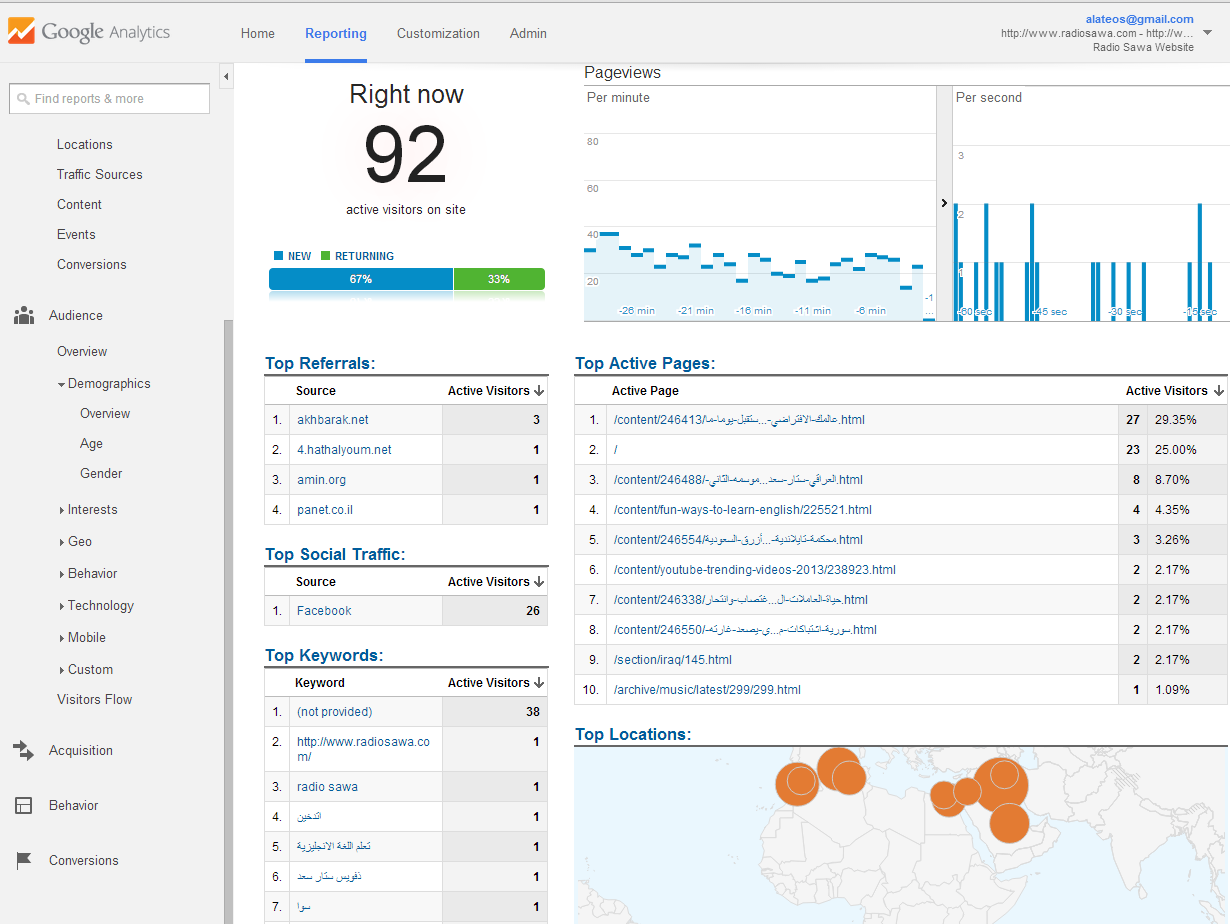
\includegraphics[scale=0.45]{img/google_analytics}
\noindent\textbf{Diagram 8 –- shows the Real-Time metrics pane in Google Analytics.} \\

As one can see, Google Analytics comes in handy in aggregating data and conveying statistical data to the end user. The end user here would navigate here with the intention of running an analysis, like: From what parts of the world is most of this website’s traffic coming from? What links are being most visited?
While this would be a great tool for management, it is unlikely that the end users will wake up to their coffee looking at this, and then navigating to the actual news website. \\

\noindent\textbf{Adobe Analytics} \\
\noindent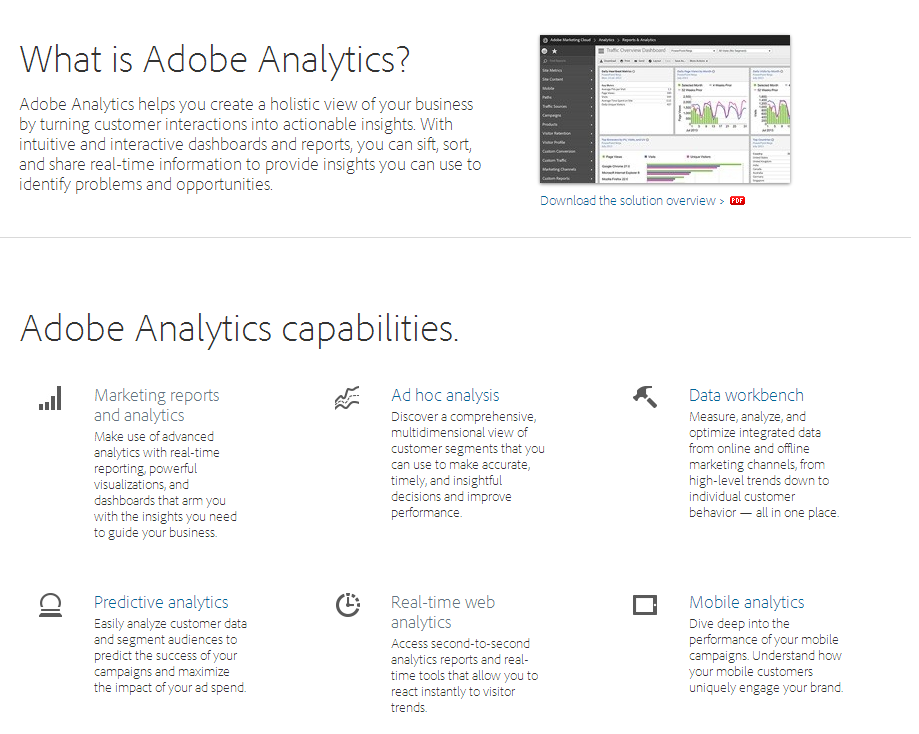
\includegraphics[scale=0.6]{img/adobe_analytics}
\noindent\textbf{Diagram 9 –- Snapshot of the Adobe Analytics landing page, which enumerates the services that Adobe Analytics encompasses.} \\

Adobe Analytics covers a slew of reporting capabilities:

\begin{itemize}
\item \textbf{Marketing reports and analytics.} Includes dashboards and reports, conveying key performance indicators, showing marketing strategies’ performance in real-time, and displaying the results of ad campaigns
\item \textbf{Ad hoc analysis.} Includes multidimensional site analysis and advanced reporting
\item \textbf{Data workbench.} Involves collecting, processing, analyzing, and visualizing Big Data from online and offline customer interactions
\item \textbf{Predictive analysis.} Pertains to discovering hidden customer behavior
\item \textbf{Real-time web analytics.} Shows what is happening on the digital properties in real-time so that managers can take action where needed
\end{itemize}

Once again, the intended audience is that of management and decision makers. The current prominent web analytics systems revolve around reporting data to the decision makers. What I plan to create is for the end users.

\null
\vfill
\section{Work Plan}
\subsection{Assumptions, Risks and Alternatives}
I will require a web host where I can test the web technologies as well as store my database. I currently am subscribed to a web host that provides me with a LAMP (Linux, Apache, MySQL, PHP) environment. This is where I plan to execute all my development and testing. The scripts technologies to be used are HTML 5, CSS3, PHP, MySQL, and JavaScript. The libraries I anticipate to use are D3 and possibly JQuery.
I can foresee the following risks:

\begin{itemize}
\item The web traffic captured will not be 100\% accurate. Then again, no web analytics system out there is perfect as of this writing, given the stateless nature of http and how http traffic is passed and downloaded over the net. My goal here is to maximize accuracy, given my research and best judgment
\item The visualization turns out to be slow due to the web browser rendering too much data at once. In this event, I will scale down the complexity of the visualization to match the current average machine's CPU power and web browser engine capabilities. Alternatively, I can utilize AJAX (where applicable) to render the required data on demand
\end{itemize}

\noindent{Basically, my strategy for mitigating any further risks will be to narrow the scope of the end product. In the lack thereof, I plan to fully capitalize on enhancing functionality.}

\subsection{Preliminary Schedule}
\begin{itemize}
\item[] \textbf{Weeks 1-3} (Research what data needs to be captured): \\
Research the metrics that need to be captured. What defines a website visit? What data will need to be collected?

\item[] \textbf{Weeks 4-6} (Design a relational database to house desired data):): \\
Here, I will define the relational schemas and will accordingly build a MySQL database that will contain all of my desired data. \\
Deliverable --- Relational database to house all data pertinent to website traffic hits.

\item[] \textbf{Weeks 7-10} (Code and implement a PHP implementation for data storing/retrieval): \\
Here, I plan to build PHP classes and functions that will connect to the database to store the web traffic data. In addition, I will write the code that will query the database in order to extract and convey meaningful data. \\
Deliverable --- Full server-side code base that collects and retrieves web traffic data.

\item[] \textbf{Weeks 10-12} (Implement mock news site): \\
Here, I plan to build a mini news site that contains several categories. Then, I will create several articles under each of the created categories. I am inclined to building this mock site in Wordpress, as it is commonplace and reflective of the archetype of your common CMS site.
Deliverable --- A mini Wordpress mock site, mimicking the structure of a news website

\item[] \textbf{Weeks 13-16} (Research and experiment with different visualizations): \\
Before I commit to a visualization, I would like to make sure that it is the most fit for my domain at hand. Thus I will test my data inside a few viable options, before fully scoping my visualization. \\
Deliverable --- An existing or custom designed visualization template to convey near real-time web traffic data.

\item[] \textbf{Weeks 16-18} (Implement final visualization): \\
Once I have selected my visualization of choice, I will code and implement it. \\
Deliverable --- A fully implemented web visualization which interacts with the server-side database.

\item[] \textbf{Weeks 18-20} (Test with users and apply final touches): \\
I will attempt to reach a wide and diverse audience for feedback. I will incorporate the meaningful feedback into my refinement iteration. "Meaningful" here represents anything significant enough to affect the usability of the visualization.

\end{itemize}

\vfill

\section{Implementation}
\subsection{Capturing Data}
\subsubsection{IP Addresses}
I plan to capture the IP addresses of the visitors to the subject news site. In PHP, an associative array called \textbf{\$\_SERVER}  contains several variables that pertain to the HTTP connection between the client and the server. The variable that contains the IP address from which the user is viewing a select page is called \textbf{REMOTE\_ADDR}. In code, we register the visiting IP address like so:
\begin{lstlisting}
$user_ip = $_SERVER["REMOTE_ADDR"];
\end{lstlisting}

Here, I would like to shed light on the difference between static and dynamic IP addresses. The former is set by the network administrator and is fixed unless it is changed manually. The latter is assigned by the network router, and is assigned for a temporary period called the DHCP lease time. In order to find out the average DHCP lease time set by Internet Service Providers (ISPs), I asked a few network engineers and contacted 3 prominent ISPs. Here are the results:
\vspace{0.3in}

\begin{tabular}{| c | c |}
  \hline                       
  Network Engineer 1 & 7 days \\[1ex] \hline
  Network Engineer 2 & 3 days \\[1ex] \hline
  Network Engineer 3 & 3 days \\ [1ex] \hline
  Verizon (ISP) & 14 days \\[1ex] \hline
  Comcast (ISP) & 4-7 days \\[1ex]
  \hline  
\end{tabular}
\vspace{0.3in}

The average DHCP lease time is between 3 and 7 days. Since in my visualization I only care for recent and breaking news that span for 1-3 days, I can hold the distinction between static and dynamic IP addresses as constant - as the time span is less than the average renew period. This is important for monitoring the average time spent on an article and other metrics that rely on graduation of time. The IP address is the only means to track a user and that does not require user authentication. 

As for user integrity, one cannot fully ensure that a physical human is sitting behind an IP address when bots, web scrapers, and other automated processes may be hitting the IP address of a given news article. Though, my goal is to minimize the inaccuracy when a visitor reaches a news article. My plan to counter this is to only register the visiting IP address when the user has moved his/her mouse, or, when he/she has scrolled at least once when viewing the article at hand. I have tested a stub for this successfully in \textbf{register\_ip.php}. Here, I have a page containing several blocks of repeated Lorem ipsum text. I used JavaScript to listen to the mousemove and scroll events. I used jQuery to shorthand the event bindings. Below is the code:
\begin{lstlisting}
mouse_moved = false;
page_scroll_counter = 0;

$("body").on("mousemove",function(){
	if(!mouse_moved) {
		\\ Here, a flag would be sent to the server via AJAX
		console.log("Mouse has moved");
		mouse_moved = true;
	} else {
		
	}
});

$(document).on("scroll",function(){
	if(page_scroll_counter == 1) {
		\\ Here a flag would be sent to the server via AJAX
		console.log("Page has been scrolled")
	} else {
		page_scroll_counter++
	}
});
\end{lstlisting}        

\subsubsection{Geographic origins}
The world is smaller than it has ever been. One of the metrics I am opting for is the user geographic distribution for a select news article. This requires two steps:
\begin{enumerate}
\item Capturing the IP address of the user. This was demonstrated in the previous section
\item Obtaining the corresponding latitude and longitude coordinates associated with the user's IP address
\end{enumerate}

Here, it is important to note that many users may be sitting behind HTTP proxy servers. HTTP proxy servers are physical computers/servers that act as proxy points for the client computers. For example, if someone in Russia used a proxy server in the US to visit my news article, the requesting IP address that will be captured will be that of the US - making it appear that the user that visited the article actually came from the US. In PHP, in addition to \textbf{\$\_SERVER["REMOTE\_ADDR"]}, there is another variable called \textbf{\$\_SERVER["HTTP\_X\_FORWARDED\_FOR"]}. While the former gets the IP address of the direct requester, the latter gets the originating IP that is making the request. So for example, if I were to be sitting behind an IP proxy server which had an address of 111.111.111.111, then \$\_SERVER["REMOTE\_ADDR"] would carry that value. \\
\$\_SERVER["HTTP\_X\_FORWARDED\_FOR"] would then contain the value of my router's outside IP address - which is what I am looking to map geographically.   
\\ If on the other hand the user was browsing the Internet normally, without the use of a proxy server, then \$\_SERVER["REMOTE\_ADDR"] would carry the value of the user's router's IP address - reflective of the user's geography. 
It will thus be a challenge to capture the needed IP address to look up geographically. Here is the methodology that I will use to capture the needed IP address for the geographic lookup:
\begin{enumerate}
\item Get the value of \$\_SERVER["REMOTE\_ADDR"] and look up its value with a geolocation API. Call this \textbf{X}
\item Get the value of \$\_SERVER["HTTP\_X\_FORWARDED\_FOR"] and look up its value with a geolocation API. Call this value \textbf{Y}
\item If X and Y are both available, it means that the user is sitting behind a proxy and that the needed IP address is that of Y. If X is available but Y is not, it means that Y is a private IP address, that of the device behind its router - and thus not behind a proxy server. In this case, X would hold the IP address of the origin.
\end{enumerate} 

The next step here is to find a service that would map a given IP address to its corresponding geo coordinates, and ideally to its country name. A quick Google search revealed a convenient REST API service that would output the responses in JSON. \textbf{Telize (www.telize.com)} is a REST API that allows one to get the visitor IP address and to query the location information for that IP address. The upside of this service is that at the moment it contains to no rate limits; thus, one could make an indefinite amount of calls to the Telize API. I was able to test the above clause 3 in PHP code with success. Regardless, of whether I was sitting behind a proxy server or not, the output showed the United States as the country of origin. Here is the code:
\begin{lstlisting}

date_default_timezone_set("America/New_York");

$remote_addr = $_SERVER["REMOTE_ADDR"];
$x_forwarded_for = $_SERVER["HTTP_X_FORWARDED_FOR"];

$url1 = "http://www.telize.com/geoip/" . $remote_addr; 
$url2 = "http://www.telize.com/geoip/" . $x_forwarded_for; 

// Get the country for the ip behind the first
// exposed remote address (from www.telize.com)
$results1 = file_get_contents($url1);
$results1 = json_decode($results1);
$country1 = $results1->country;

// Get the country for the ip behind the second
// exposed remote address (from www.telize.com)
$results2 = file_get_contents($url2);
$results2 = json_decode($results2);
$country2 = $results2->country;

$final_country = "";

if(strlen($country1) > 0 && strlen($country2) > 0) {
	echo "User is most likely behind a proxy server.<br />"; 
	$final_country = $country2;
} else {
	echo "User is not behind a proxy server.<br />";
	$final_country = $country1;
}

echo "The user's country of origin is " . $final_country;

\end{lstlisting}   

\subsubsection{Average Read Time}

One metric that I would be curious to attain is how long the average user spends reading a certain news article. At the moment, a cousin measure called the bounce rate checks to see whether the user continues to browse other pages in the site, or whether the user 'bounces' off to other websites. Naturally, this measure is not indicative of the level of interest the reader has for a given news article. I plan to get this by doing the following:
\begin{enumerate}
\item Research the average reading speed of adults that can read English
\item Count the number of words in a given news article
\item Based on the average read speed, calculate the time spent on the news article. If the page is kept open indefinitely by the reader, I will simply use the maximum expected read time for that article. While this is in no way 100\% accurate, it will be highly reflective of the level of interest with the visited articles. 
\end{enumerate}     

\noindent Based on an ophthalmology study that consisted of 50 native English-speaking individuals (average age 30.38$\pm$9.44 years; 16 university students, 18 academics, and 16 non-academics) -- the average reading speed came out to be 201.53$\pm$35.88 words per minute(wpm) for short sentences, and 215.01$\pm$30.37 wpm for long paragraphs\cite{radner}. For the scope of this project, I will use the average of 200 wpm to calculate the maximum average time spent on a news article.  

\vfill

\subsection{Database Design}
\subsubsection{Data Storage}
Based on the data that will need to be captured, below are the fields that should be created:
\begin{itemize}
\item \textbf{Visitor IP address}: This will basically store the IP address of the visitor reading the news article. In order to avoid capturing page refreshes as new sessions, I will set a threshold of 10 minutes - whereby the server checks if the visitor has visited the article in the past 10 minutes
\item \textbf{Time Visited}: This should store a timestamp (in GMT) of when the user visited 
\item \textbf{Timezone}: This will be helpful in determining time differences from GMT
\item \textbf{Country}: This will store the name of the country where the visitor is from
\item \textbf{Region}: Region pertains to the area within the country where the visitor is from
\item \textbf{Read Time}: This will store the time taken for the reader to have finished reading the article. This should be calculated in seconds
\item \textbf{Article ID}: This will be the unique identifier and should be captured as is from the host's CMS. This way, future references could be made easily without having to go through matching algorithms
\item \textbf{Category ID}: This will be the unique identifier of the category, also as it appears in the corresponding CMS
\item \textbf{Article URL}: this will be needed to enable the user to navigate through the visualization to the intended article
\item \textbf{Article title}: The title of the article as it appears in the CMS or on the news site
\item \textbf{Sample text}: In the visualization, some of the text from the body will be excerpted upon the user hovering on a select article
\item \textbf{Sample picture}: In the visualization, the user will need to see a preview pic of the article when applicable 

\end{itemize}

\subsubsection{Database Tables}
Here, I will adhere to the principles of relational database normalization in order to maximize efficiency and eliminate redundancy. For the scope of this project, all the data pertinent to a web hit can be stored in a single table: \\ 
{\large\textbf{hit (\underline{id},ip, time\_visited, \textit{article\_id}, timezone, country, region, read\_time)}} \\ \\
The underline signifies the primary key. The primary key is the field(s) that are enough to determine the rest of the information for any row instance. In this case, the IP address, article ID, and time of visit jointly determine the timezone, country, region, and read time. However, since I need a way to track the user's visits to capture read time, I have designated an auto-increment unique identifier called \textbf{id}. \textit{article\_id} is italicized since it is a foreign key -- that is, it represents a primary key in another table. The time visited will be abstracted to hour:minute. Therefore, seconds will not be accounted for in the visit's time stamp. The read time will default to the maximum read time as calculated by the article's length. This assumes that the user will stay on the article page indefinitely. In the event that the user does leave the page, this value would then register the actual read time.
\\ \\
The second table needed will contain all the metadata pertinent to the visited article:\\
{\large\textbf{article (\underline{article\_id}, category\_name, article\_url, title, sample\_text, sample\_pic)}} \\ \\

The third table needed will contain metadata pertinent to the category of the visited article:\\
{\large\textbf{category (\underline{category\_id}, category\_name})}
\\ \\

It is important to note here that all of this data will be communicated via the server side script which will be embedded in each loaded article. 

\subsubsection{MySQL Database}
For this project, I will be using MySQL since I have good experience with it and for its being open source. MySQL is a relational database management system. Relational databases are those that adhere to relational database design, which relies on the fundamentals of relational algebra and relational calculus. The main tenet of relational design is to maximize efficiency and eliminate any redundancy in the data being stored.

I created a database called \textbf{alaini\_news\_viz} on my web host. For this, I created two users:\\
\begin{itemize}
\item \textbf{alaini5\_newsread}: This account will be solely used to read from the database. Ultimately, it will be used to invoke the visualization by the visitor/end user
\item \textbf{alaini5\_newsedit}: This account will mainly be used to register the IP hits and read times communicated to the server
\end{itemize}

I created 3 tables in MySQL using phpMyAdmin, an open source PHP based GUI that facilitates interacting with the MySQL system:
\begin{enumerate}
\item{\textbf{article}}\\ \\
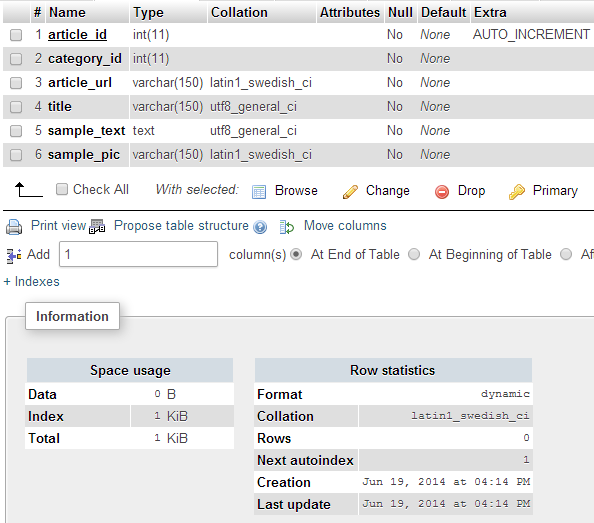
\includegraphics[scale=0.6]{img/article_table}
\item{\textbf{category}}\\ \\
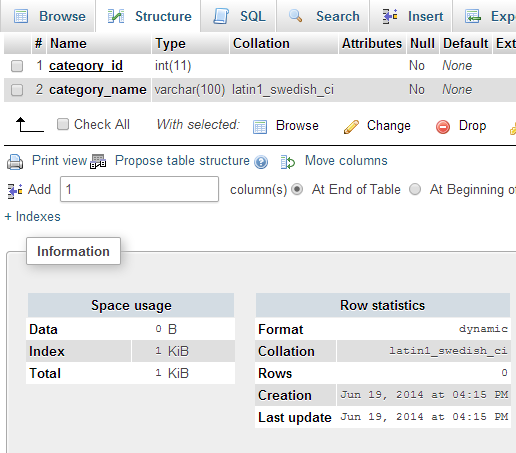
\includegraphics[scale=0.6]{img/category_table}
\item{\textbf{hit}}\\ \\
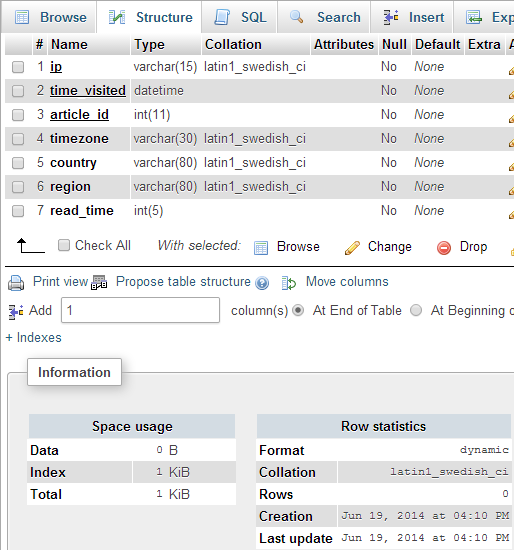
\includegraphics[scale=0.6]{img/hit_table}
\end{enumerate} 

\subsection{PHP server-side code}
\subsubsection{Configuration and database connection}
Here, I created two files:
\begin{enumerate}
\item{\textbf{constants.php:}} Holds all the constants that will be defined across the application, inclusive of those for the database connection
\item{\textbf{db\_connect.php:}} Performs the PDO database connection based on the given connection parameters
\end{enumerate}
Note that both of these files are stored one directory above \textbf{public\_html/} for security reasons. This folder is called \textbf{lib/}. Thus, the two files are not accessible directly to the public and accordingly need to be included in other PHP files.

\subsubsection{Server-side hit capture}


\vfill

\section{Glossary}
\begin{itemize}
\item[] \textbf{Apache HTTP Server (aka Apache)}: A web server software program
\item[] \textbf{Choropleth map}: A thematic map in which areas are shaded or patterned in proportion to the measurement of the statistical variable being displayed on the map (source: Wikipedia).
\item[] \textbf{Class}: In object oriented programming parlance, it refers to the abstraction and representation of a real life object or concept in code.
\item[] \textbf{CSS}: A styling language used to define the aesthetics of elements in a web deliverable. This is implemented in all major web browsers. CSS3 is the most recent version of this language.
\item[] \textbf{D3.js}: A JavaScript library for manipulating documents based on data using HTML, SVG and CSS (source: d3js.org).
\item[] \textbf{Google Analytics}: A service offered by Google that generates detailed statistics about a website's traffic and traffic sources and measures conversions and sales (source: Wikipedia).
\item[] \textbf{HTML 5}: The most recent specification for the markup language that constitutes the visual elements of any web deliverable. It also normally includes some JavaScript and CSS 3 code as part of its implementation.
\item[] \textbf{JavaScript}: A client-side scripting language that is used by all prominent web browsers.
\item[] \textbf{JSON (JavaScript Object Notation)}: A lightweight data-interchange format (source: json.org).
\item[] \textbf{LAMP}: A web development environment comprised of a Linux server, Apache HTTP Server, MySQL, and PHP.
\item[] \textbf{MySQL}: An open source relational database management system.
\item[] \textbf{Object oriented programming}: A programming paradigm that represents real-life elements and concepts as "objects". The implementation involves mimicking only the needed real-life characteristics of the object in code, and calling a working copy of these objects an "instance".
\item[] \textbf{PHP}: An open source server-side scripting language.
\item[] \textbf{Relational database}: A database built on principles of the relational model. Such a database is comprised of tables and fields.
\item[] \textbf{SVG}: An XML-based vector image format for two-dimensional graphics that has support for interactivity and animation (source: Wikipedia).
\item[] \textbf{Web visualization}: A visual deliverable created using web technologies. More than often, it is dynamic in that it visually changes based on the data being fed to it. 
\end{itemize}

\vfill

\begin{thebibliography}{1}

  \bibitem{schumann} Schumann, H. and M¨uller, W. (2000). {\em Visualisierung – Grundlagen und allgemeine Methoden}. Springer, Berlin, Germany.

  \bibitem{tufte}  Edward R. Tufte, {\em Visual Display of Quantitative Information} (2001).

  \bibitem{munzner} Munzner, T. (2009), {\em A Nested Model for Visualization Design and Validation}.

  \bibitem{cockburn} A. Cockburn, A. Karlson, and B. B. Bederson, {\em “A review of overview+detail, zooming, and focus+context interfaces,”} ACM Computing Surveys (CSUR), vol. 41, no. 1, pp. 1–31, 2008.
  
  \bibitem{playfair} Playfair, W. and Corry, J. (1786). {\em The Commercial and Political Atlas: Representing, by Means of Stained Copper-Plate Charts, the Progress of the Commerce, Revenues, Expenditure and Debts of England during the Whole of the Eighteenth Century.} printed for J. Debrett; G. G. and J. Robinson; J. Sewell; the engraver, S. J. Neele; W. Creech and C. Elliot, Edinburgh; and L. White, London, UK.
  
  \bibitem{frank} Frank, A. U. (1998). {\em Different Types of “Times” in GIS. In Egenhofer, M. J. and Golledge, R. G., editors, Spatial and Temporal Reasoning in Geographic Information Systems}, pages 40–62. Oxford University Press, New York, NY, USA.
  
  \bibitem{goralwalla} Goralwalla, I. A., O¨ zsu, M. T., and Szafron, D. (1998). {\em An Object-Oriented Framework for Temporal Data Models. In Etzion, O. et al., editors, Temporal Databases: Research and Practice}, pages 1–35. Springer, Berlin, Germany.
  
  \bibitem{bettini} Bettini, C., Jajodia, S., and Wang, X. S. (2000). {\em Time Granularities in Databases, Data Mining, and Temporal Reasoning}. Springer, Secaucus, NJ, USA, 1st edition.

  \bibitem{radner} Radner, W., Diendorfer, G., (2014). {\em English sentence optotypes for measuring reading acuity and speed --- the English version of the Radner Reading Charts}

  \end{thebibliography}

\end{document}
